\chapter{Results} \label{results}
The results of the MCMC analysis as well as the MAP optimization is visualised in the section below.
\section{Continuous output}
To assess the progress of the MCMC analysis while iterating, graphs similar to those in Figure \ref{fig:10} were continuously generated. 
In Figure \ref{fig:10} the output of 2000 iterations were extracted to allow sufficient detail to be visible.
Figure \ref{fig:10a} was important to keep track of the number of different samples assessed until an acceptable sample was found.
If a large number of samples were consistently needed, it could indicate that a bad starting point was chosen or that there is an error within the posterior distribution calculation.
The connection between Figures \ref{fig:10b} and \ref{fig:10c} can be seen in that when there is a dip in the difference between $\pi^*(x)$ and $\pi^*(x_{\text{ref}})$ there is a peak in the acceptance ratio.
When the graph in Figure \ref{fig:10b} is at 0 that means that the sampled values are the same as the Eurocode reference values.
When this graph is below 0 that indicates that the values sampled for that iteration produced a less likely result than the reference values.
This influenced the burn-in period chosen, to ensure that all the samples considered were more accurate than the Eurocode values.
As the probability function used is not normalised it can produce posterior probabilities larger than 1 therefore the difference between two posterior can also be larger than 1.
This also means that the higher the difference between $\pi^*(x)$ and $\pi^*(x_{\text{ref}})$ the more accurate the $x$ value is.

\begin{figure}
	\centering
	
	\begin{subfigure}[b]{\textwidth}
	\centering	
	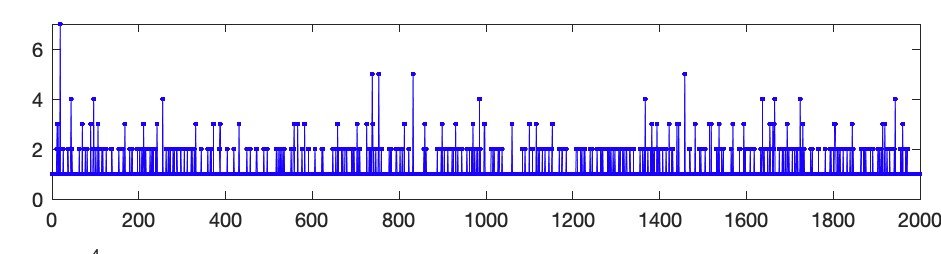
\includegraphics[width = \textwidth]{figures/figure10a.jpg}
	\caption{Number of samples drawn before an acceptable sample was found per iteration}
	\label{fig:10a}
	\end{subfigure}{}
	
	\begin{subfigure}[b]{\textwidth}
	\centering	
	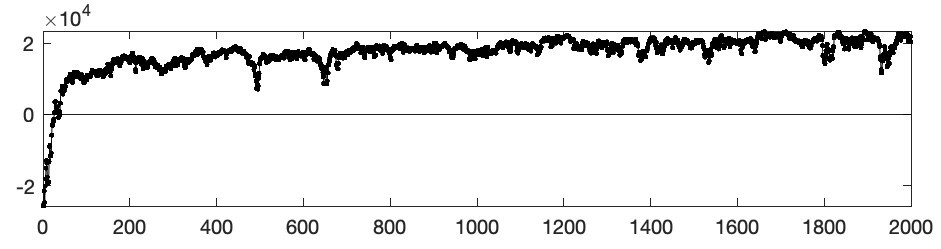
\includegraphics[width = \textwidth]{figures/figure10b.jpg}
	\caption{Difference between the accepted $x$ posterior and the reference posterior for each iteration}
	\label{fig:10b}
	\end{subfigure}{}
	
	\begin{subfigure}[b]{\textwidth}
	\centering	
	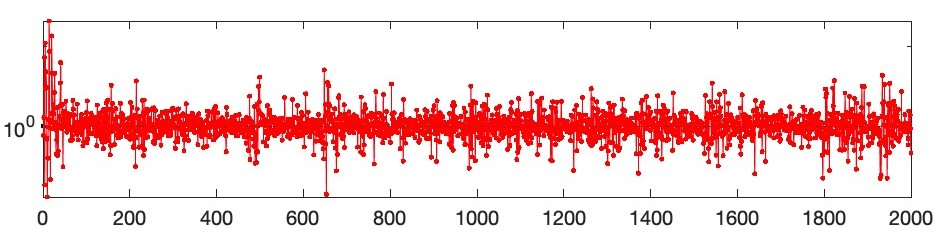
\includegraphics[width = \textwidth]{figures/figure10c.jpg}
	\caption{Value of acceptance ratio at each iteration}
	\label{fig:10c}
	\end{subfigure}{}
	
	\caption{Graphs from continuous output}
	\label{fig:10}
\end{figure}



\section{Resulting \texorpdfstring{$\kappa$}{TEXT}-values}

The thermal conductivity ($\kappa$-values) at key temperatures integral to this project, the resulting values are shown in Table \ref{krestab}. 
As can be seen in Figure \ref{kresult_euro_fig} there was quite a drastic difference in the thermal diffusivity at 1200 \textdegree C and between 0\textdegree C and 200\textdegree C.
The large difference at 1200\textdegree C is due to how the model is created, at that temperature the majority of the heat is transferred through thermal radiation.
The model did not model thermal radiation separately but instead incorporated the radiation into a equivalent conduction.
Between 0\textdegree C and 200\textdegree C the modelling of the evaporation was moderately successful as a spike can be seen at 100 \textdegree C.  
\begin{figure}
\centering	
	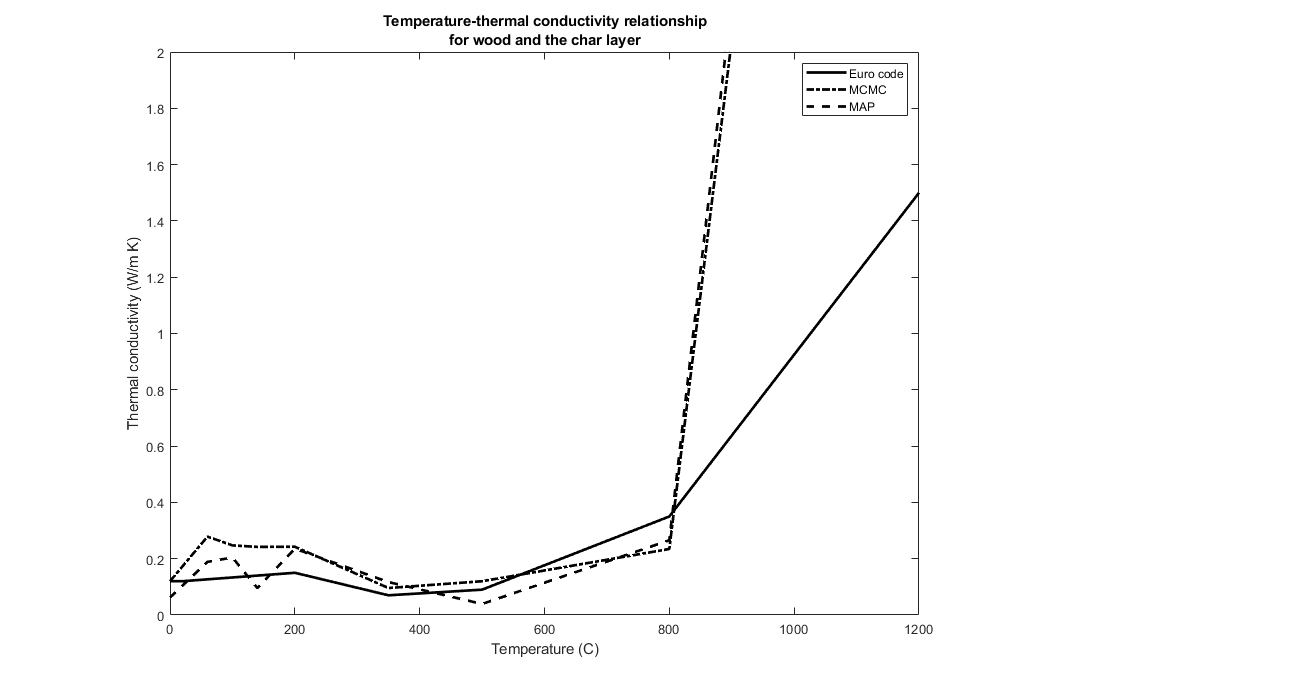
\includegraphics[width=\textwidth]{figures/kvalues_all_NOshi.png}
	\caption{Resulting $\kappa$ values compared to Eurocode standard values}
	\label{kresult_euro_fig}
\end{figure}
\begin{table} 
\centering
\caption{Posterior thermal conductivity in W/(m$\cdot$K)}
\label{krestab}
	\begin{tabular}{ r r r r }
	\toprule
	 \textdegree C & EURO & MAP & MCMC\\
	\midrule
	0   & 0.12&0.062 &0.12\\
	60  &0.12& 0.189 &0.278\\
	100 &0.12& 0.204 &0.247\\
 	140 &0.12& 0.096 &0.242\\
	200 & 0.15& 0.236 &0.243\\
	350 & 0.07& 0.117  &0.096\\
	500 & 0.09& 0.039 &0.120\\
	800 & 0.35& 0.265 &0.234\\
	1200& 1.5& 7.943 &7.467\\
	\bottomrule	
	\end{tabular}
	
\end{table}
 
 For each temperature there will be a different distribution of samples. 
 In Figure \ref{fig:scatdata} The distribution of all the samples were plotted in a scatter plot.
 The resulting $\kappa$-values from the MCMC algorithm is plotted in red and the Maximum a posteriori is plotted in blue.
 The non-symmetrical distribution  is clear in the data as the Maximum a posteriori is not in the centre of each distribution.

%TODO
From the difference between the histogram maximum and the maximum found by the Nelder-Mead optimization at 140\textdegree C (Figure \ref{fig:histo}) it is clear that many more iterations of the MCMC algorithm is needed.
In contrast at 60\textdegree C the maximum of the histogram and the MAP is the the same indicating that the samples at that specific temperature was sufficiently explored.
An estimated 100 000 iterations would be needed.
As the current iterations already took four days an additional sixteen days would have been needed to generate the needed additional samples.
This would have been impractical to achieve during a single semester as these iterations needed the full computational capacity of the available laptop and prevented any other usage of the laptop.

\begin{figure}

\centering
	\begin{subfigure}[b]{0.45\linewidth}
	\centering
	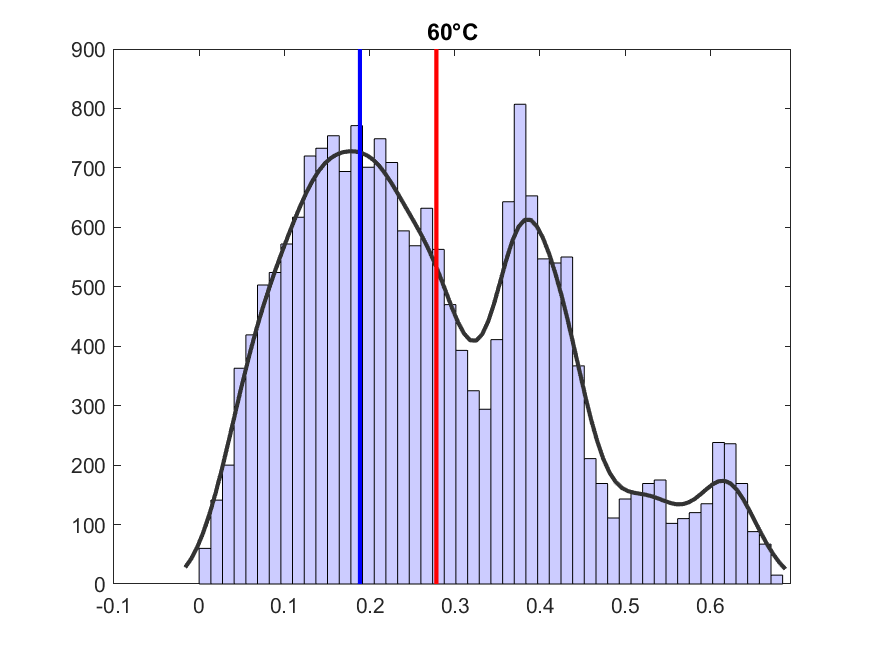
\includegraphics[width = \linewidth]{figures/histograph/histo1.png}
	\end{subfigure}
	\begin{subfigure}[b]{0.45\linewidth}
	\centering
	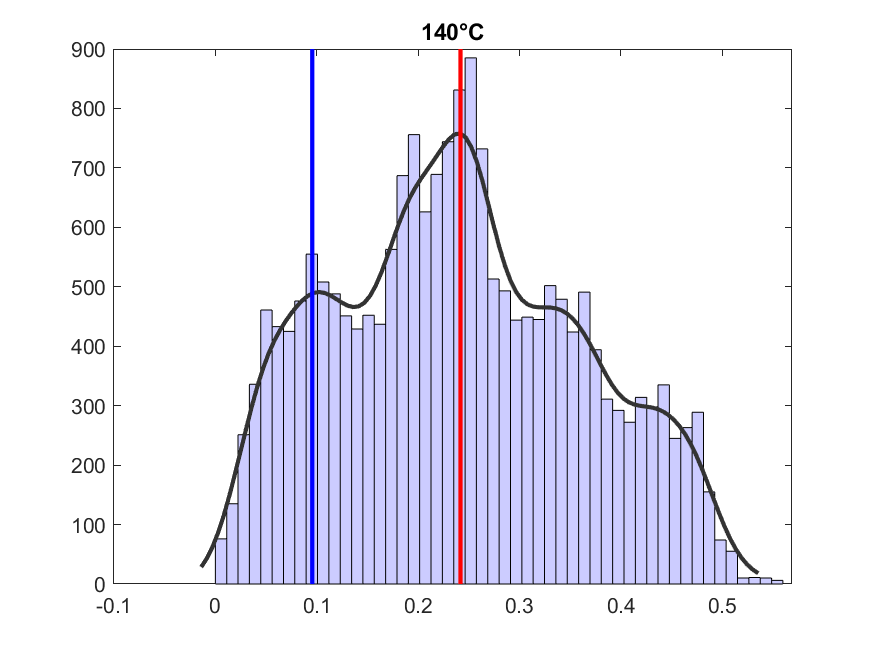
\includegraphics[width = \linewidth]{figures/histograph/histo3.png}
	\end{subfigure}
	\centering
	\begin{subfigure}[b]{0.2\linewidth}
	\centering
	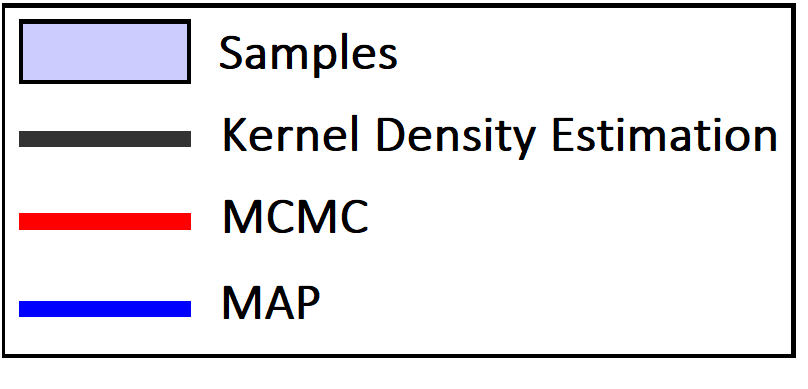
\includegraphics[width = \linewidth]{figures/histograph/legend.png}
	\end{subfigure}
	\caption{Distribution of samples at 60\textdegree C and 140\textdegree C with MCMC and MAP results indicated}
	\label{fig:histo}
\end{figure}

%\begin{figure}[b]
\label{histofig}
\centering
	\begin{subfigure}{}
	\centering
	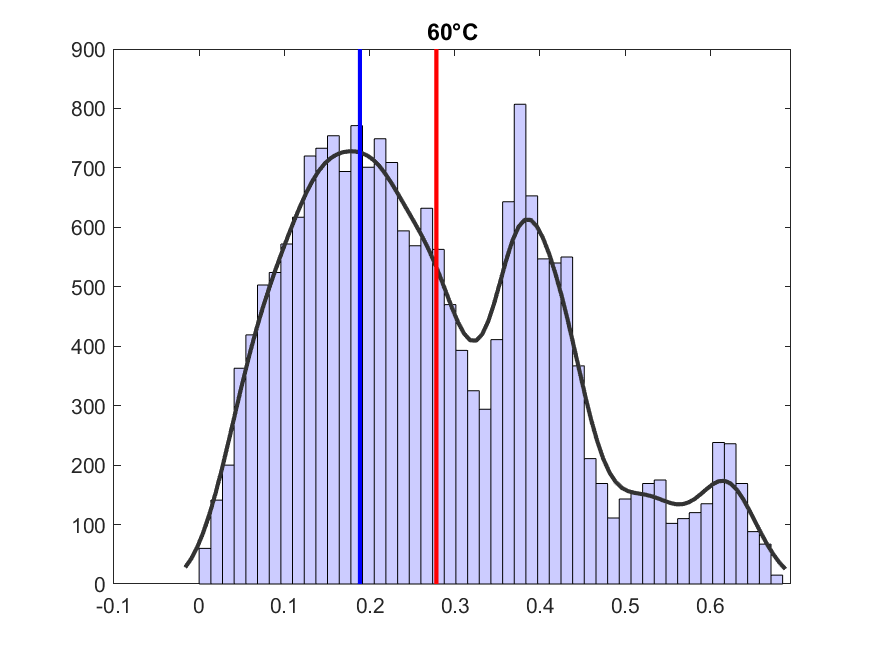
\includegraphics[width = 0.45\linewidth]{figures/histograph/histo1.png}
	\end{subfigure}
	\begin{subfigure}{}
	\centering
	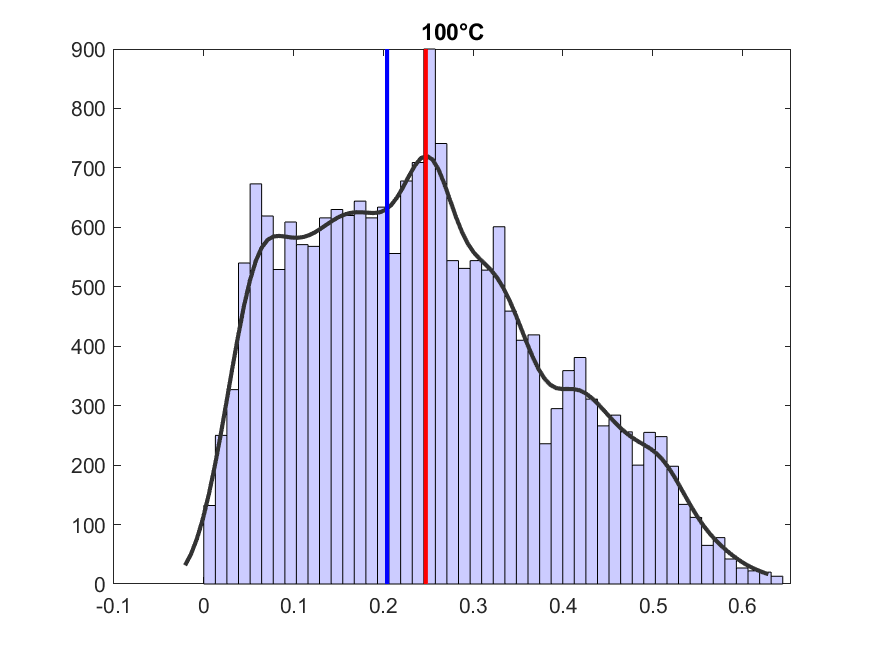
\includegraphics[width = 0.45\linewidth]{figures/histograph/histo2.png}
	\end{subfigure}
	\begin{subfigure}{}
	\centering
	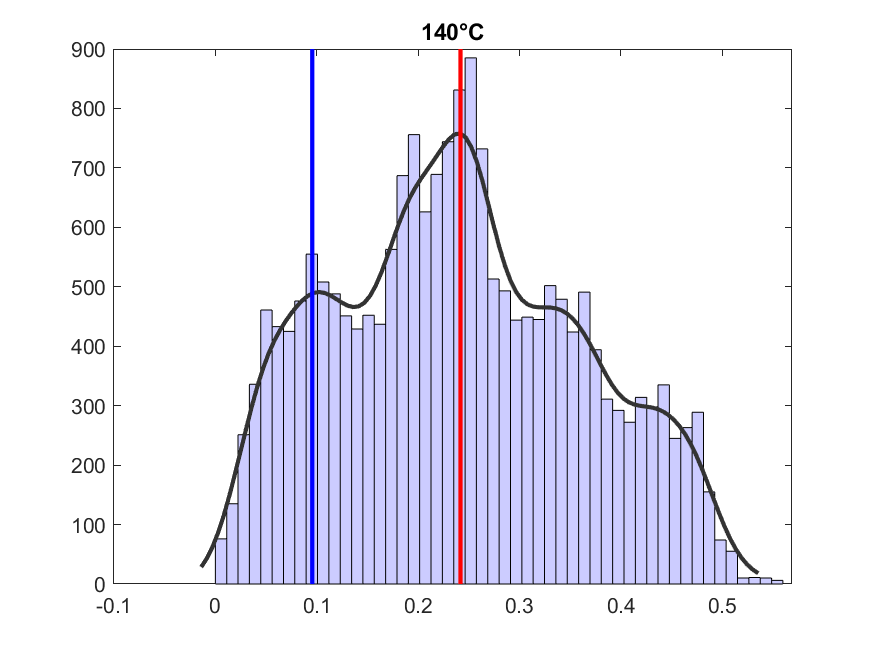
\includegraphics[width = 0.45\linewidth]{figures/histograph/histo3.png}
	\end{subfigure}
	\begin{subfigure}{}
	\centering
	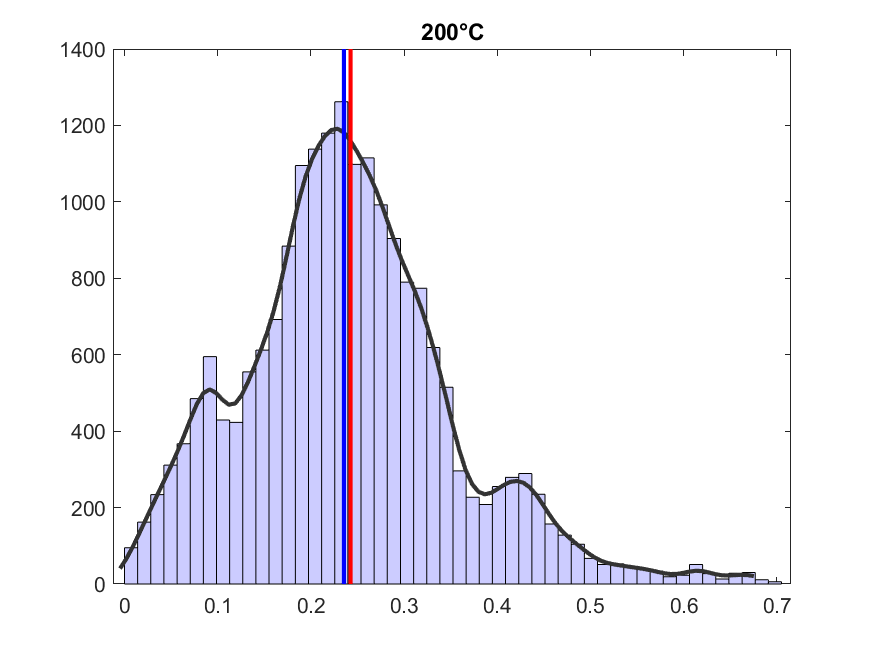
\includegraphics[width = 0.45\linewidth]{figures/histograph/histo4.png}
	\end{subfigure}
	\begin{subfigure}{}
	\centering
	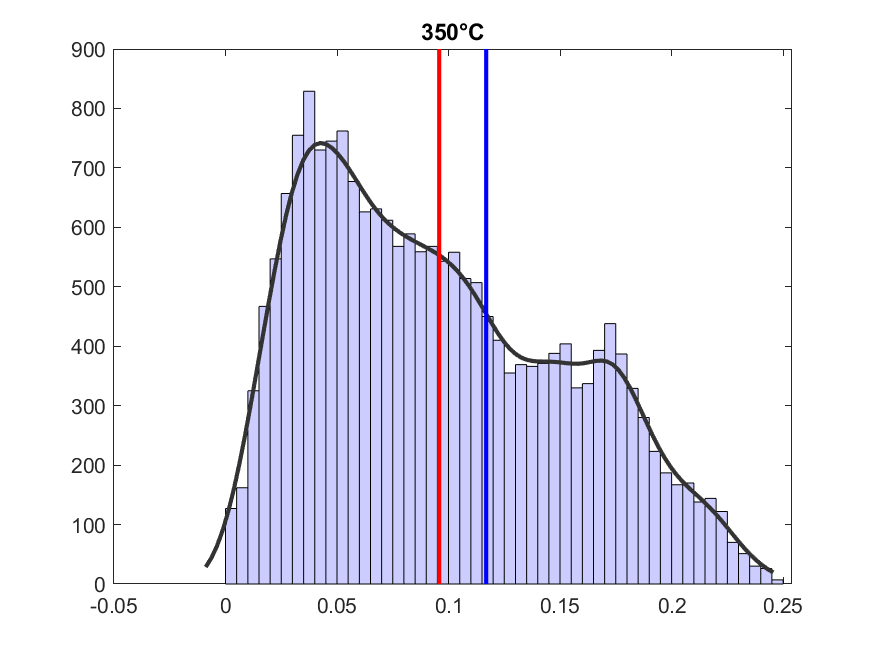
\includegraphics[width = 0.45\linewidth]{figures/histograph/histo5.png}
	\end{subfigure}
	\begin{subfigure}{}
	\centering
	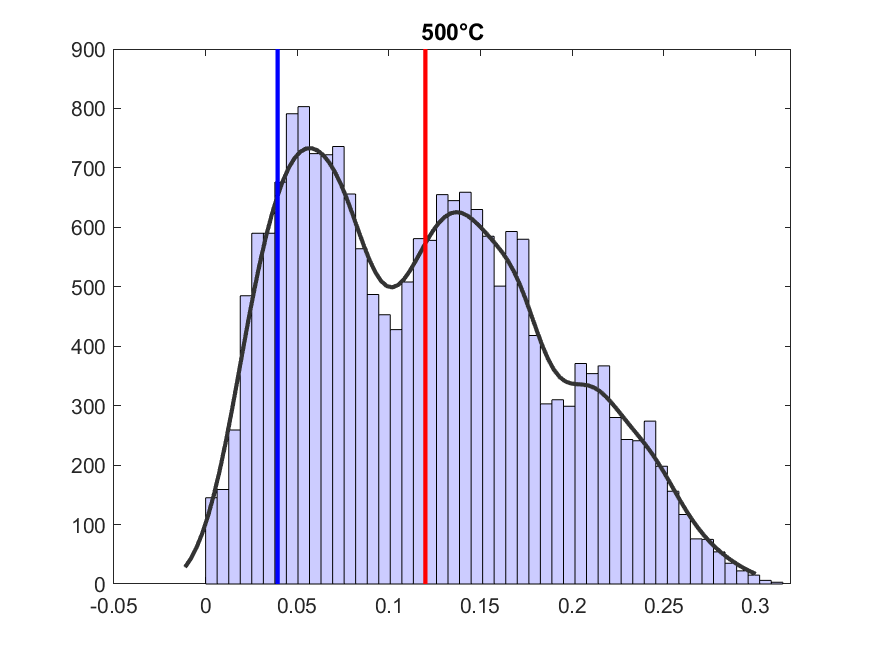
\includegraphics[width = 0.45\linewidth]{figures/histograph/histo6.png}
	\end{subfigure}
	\begin{subfigure}{}
	\centering
	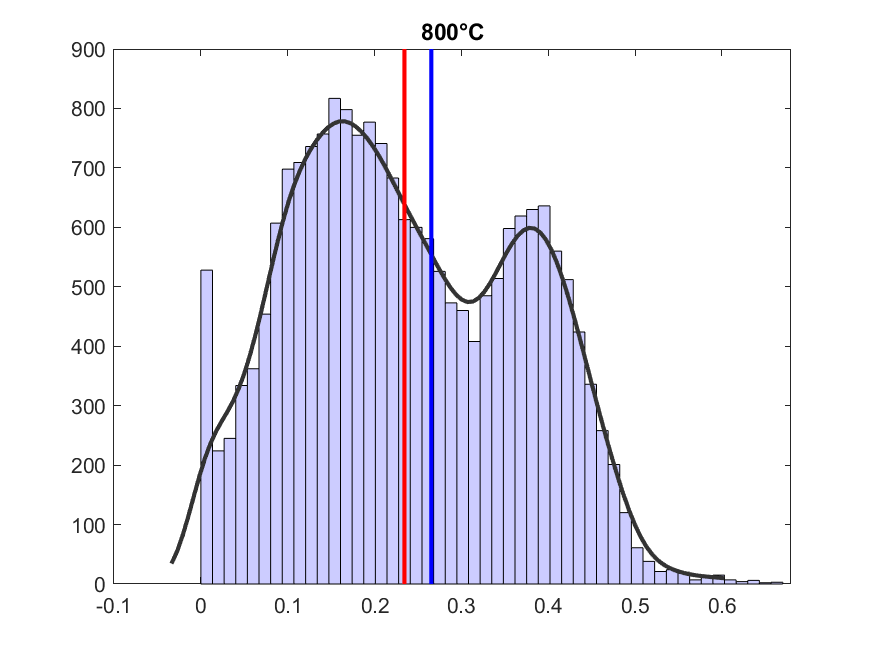
\includegraphics[width = 0.45\linewidth]{figures/histograph/histo7.png}
	\end{subfigure}
	\begin{subfigure}{}
	\centering
	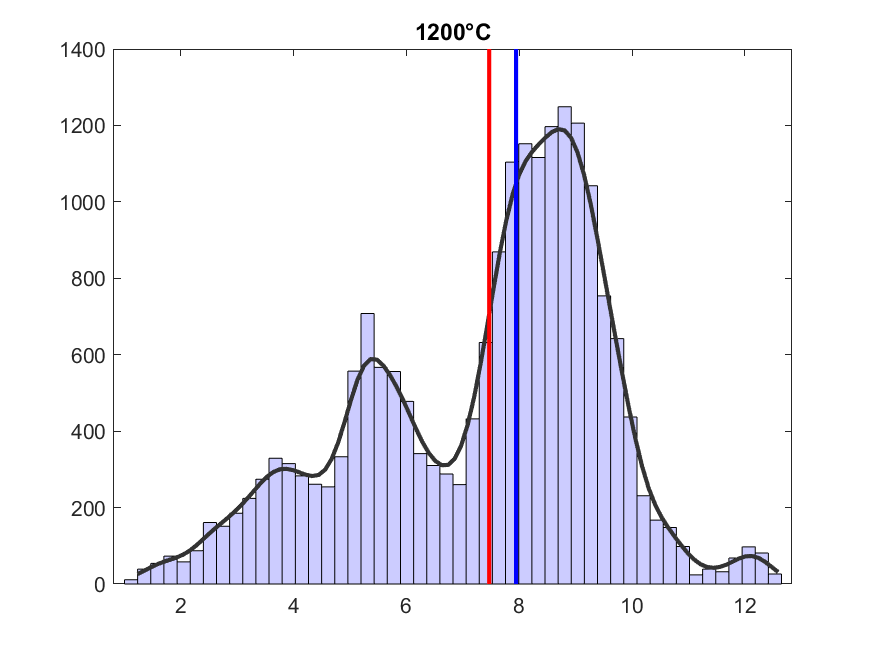
\includegraphics[width = 0.45\linewidth]{figures/histograph/histo8.png}
	\end{subfigure}
	\centering
	\begin{subfigure}{}
	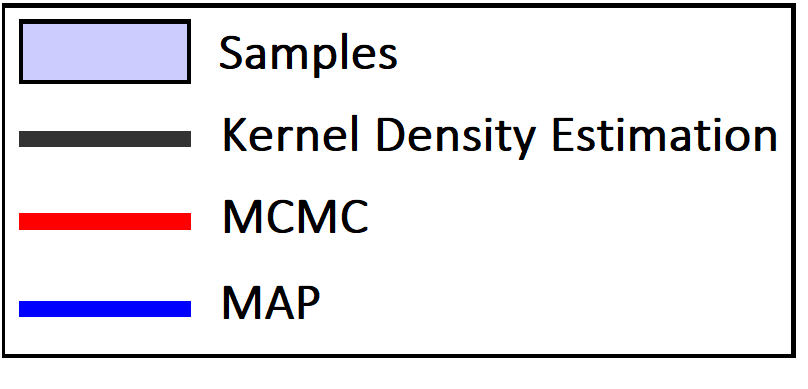
\includegraphics[width = 0.3\linewidth]{figures/histograph/legend.png}
	\end{subfigure}
	\caption[short]{Distribution of samples at different temperatures with MCMC and MAP results indicated}
\end{figure}
\begin{figure}[b]
\label{fig:scatdata}
\centering
	\begin{subfigure}{}
	\centering
	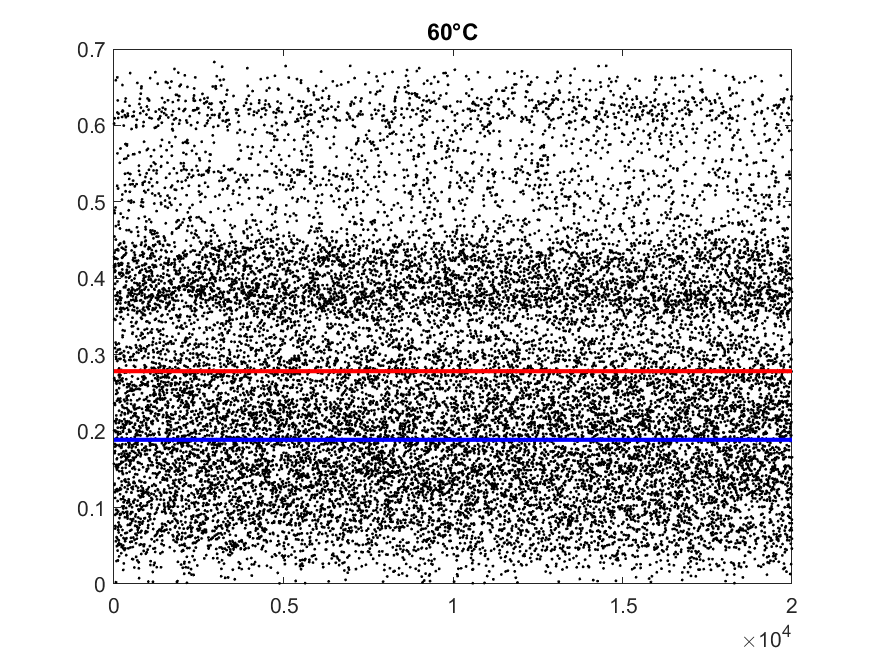
\includegraphics[width = 0.45\linewidth]{figures/histograph/scatter1.png}
	\end{subfigure}
	\begin{subfigure}{}
	\centering
	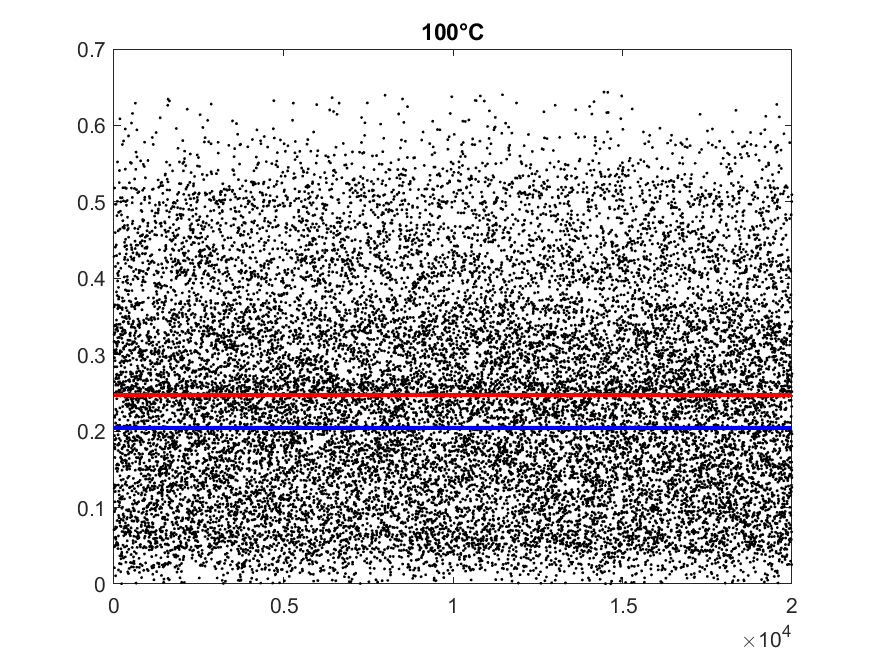
\includegraphics[width = 0.45\linewidth]{figures/histograph/scatter2.png}
	\end{subfigure}
	\begin{subfigure}{}
	\centering
	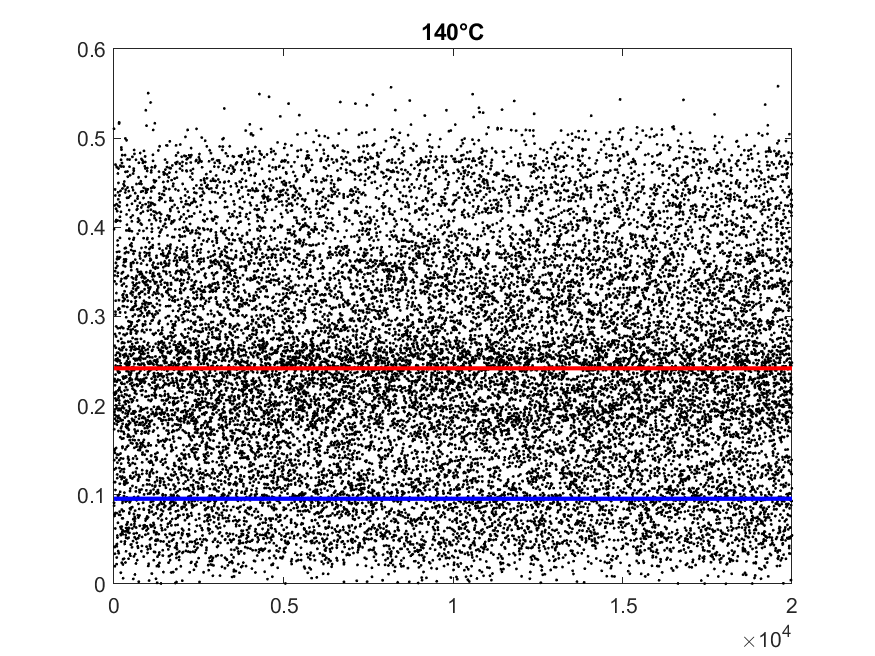
\includegraphics[width = 0.45\linewidth]{figures/histograph/scatter3.png}
	\end{subfigure}
	\begin{subfigure}{}
	\centering
	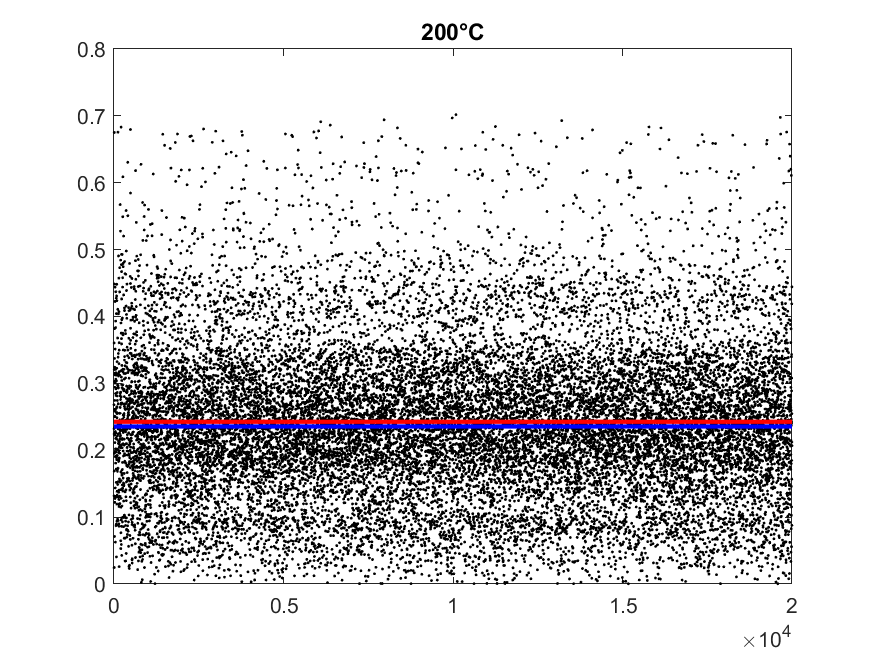
\includegraphics[width = 0.45\linewidth]{figures/histograph/scatter4.png}
	\end{subfigure}
	\begin{subfigure}{}
	\centering
	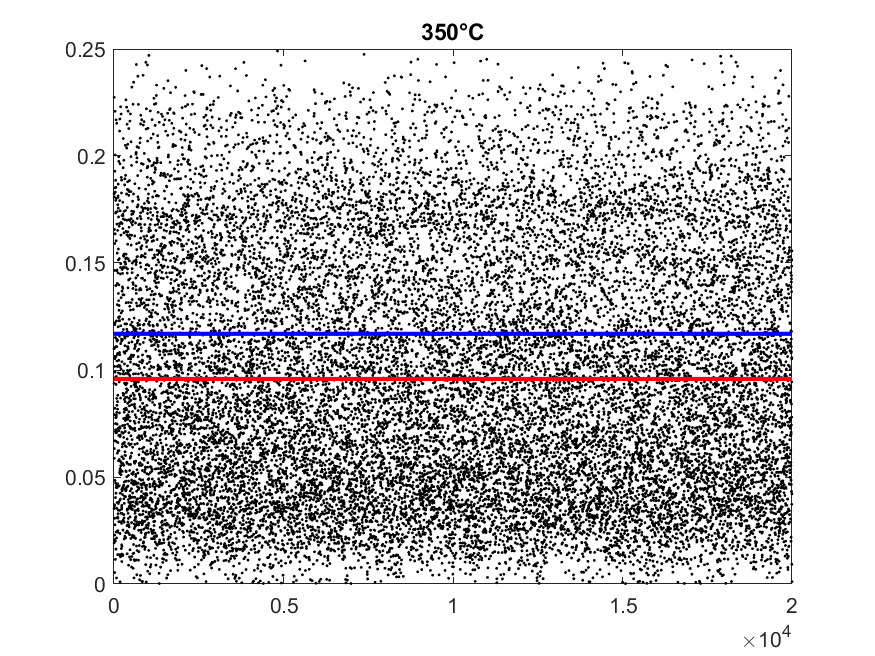
\includegraphics[width = 0.45\linewidth]{figures/histograph/scatter5.png}
	\end{subfigure}
	\begin{subfigure}{}
	\centering
	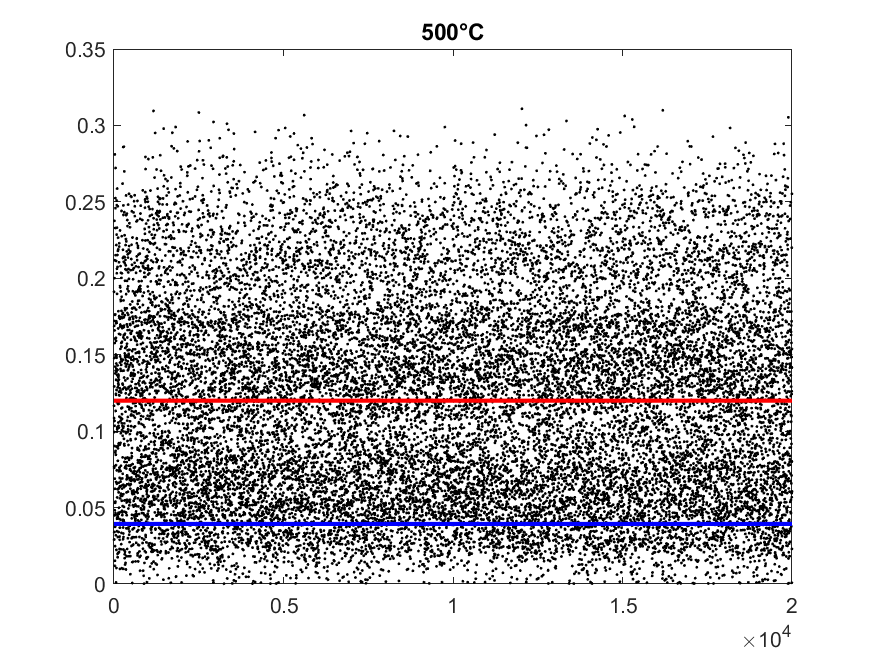
\includegraphics[width = 0.45\linewidth]{figures/histograph/scatter6.png}
	\end{subfigure}
	\begin{subfigure}{}
	\centering
	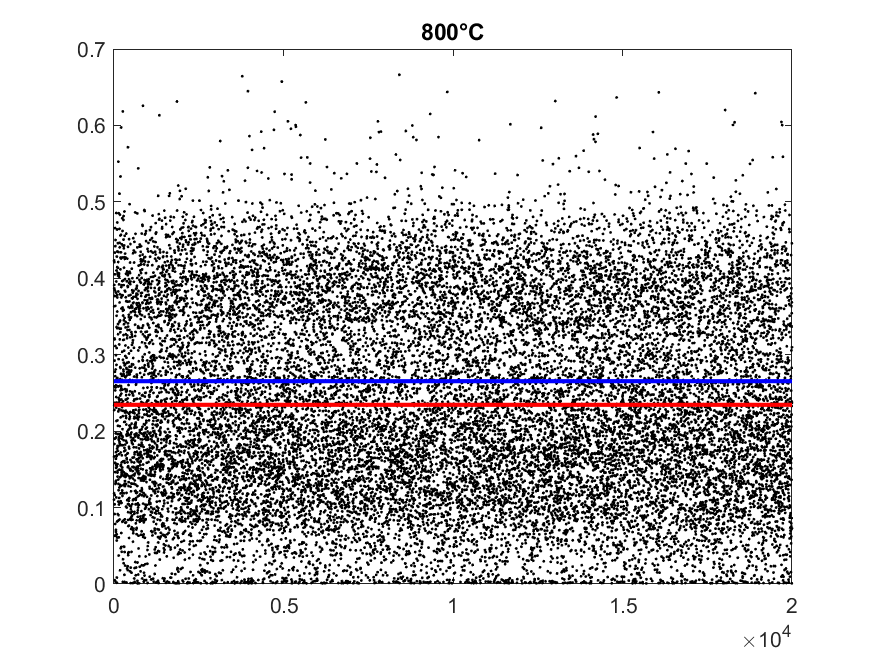
\includegraphics[width = 0.45\linewidth]{figures/histograph/scatter7.png}
	\end{subfigure}
	\begin{subfigure}{}
	\centering
	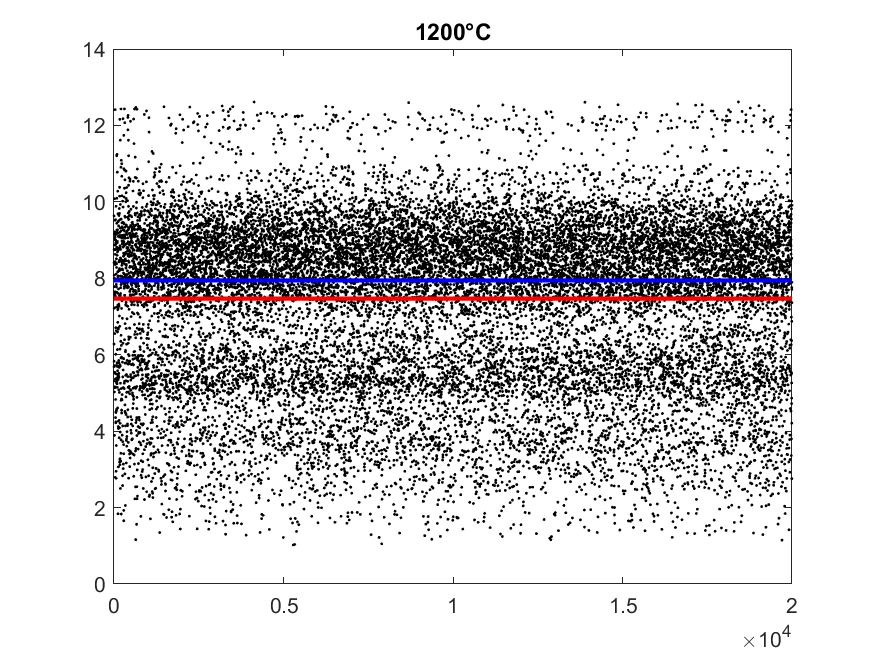
\includegraphics[width = 0.45\linewidth]{figures/histograph/scatter8.png}
	\end{subfigure}
	\centering
	\begin{subfigure}{}
	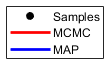
\includegraphics[width = 0.2\linewidth]{figures/histograph/scatter_legend.png}
	\end{subfigure}
	\caption{Distribution of samples at different temperatures with MCMC and MAP results indicated}
\end{figure}

\subsection{Evaluation of error}
Despite the uncertainties connected to the problem, a quantifiable measure of error is still required to allow unbiased assessment of the success of the algorithm and results.
The obtained $\kappa$-values will be used to rerun the model and obtain the new modelled temperature for each depth. 
For each depth the error will be quantified using the norm of the relative error at the seven different depths, denoted as $i$.
The relative error will be calculated according to  Equation \ref{relerror}. 
The new modelled output errors are compared to the Eurocode $\kappa$-value output errors to assess if the methods used produced a more accurate representation of the data.
The error at different depths are summarised in Table \ref{errortab} and the lowest error at that depth is highlighted in green. 
At a depth of 0mm none of the errors are highlighted as this temperature is independent of the $\kappa$-values.
This error measurement can be used to asses the error in the model or assumptions made to obtain the model.
It is important to note that this error does not only quantify the error in the thermal conductivity but any errors due to model assumptions are also encompassed.

\begin{equation}\label{relerror}
\epsilon _i = \frac{\norm{\hat{x}_i-x_i }_2}{\norm{x_i}_2} \quad \quad i= 1, ... ,7
\end{equation}

\begin{table}[H] 
\centering
\caption{Summary of error between models and data}
\label{errortab}
	\begin{tabular}{ r r r r }
	\toprule
	Depth(mm) & EURO & MAP & MCMC\\
	\midrule
	0 & 0.289 & 0.289 & 0.289\\
	16.5 & 0.217 & \cellcolor{green!20}0.194 & 0.205\\
	33 & 0.301   & \cellcolor{green!20} 0.191 & 0.200\\
	49.5 & 0.569 & 0.348 &\cellcolor{green!20} 0.323\\
	66 & 0.547   & 0.316 & \cellcolor{green!20}0.267\\
	82.5 & 0.501 &\cellcolor{green!20} 0.339 & 0.358\\
	99 & 0.219   & 0.219 &\cellcolor{green!20} 0.219\\
	\bottomrule	
	\end{tabular}
	
\end{table}

\subsection{Thermal diffusivity}
The main intent of this project was to determine the thermal diffusivity of SA-Pine. 
In Table \ref{diffrestab} the resulting thermal diffusivity is shown.
The thermal diffusivity was calculated using the information in Table \ref{cptab} and Equation \ref{alphaeq}.

\begin{table}[H]
\centering
	\caption{Resulting thermal diffusivity($\alpha \ten{-4}$)in m/s$^2$ }
	 \label{diffrestab}
	\begin{tabular}{ r r r r }
	\toprule
	Temp \textdegree C & EURO & MAP & MCMC\\
	\midrule
	0&   $1.64$&	$0.85$&	$1.64$\\
	60&  $1.64$&	$2.58$&	$3.79$\\
	100& $1.64$&	$2.78$&	$3.37$\\\
	140& $1.64$&	$1.31$&	$3.30$\\
	200& $2.05$&	$3.21$&	$3.32$\\
	350& $0.96$&	$1.60$&	$1.31$\\
	500& $1.23$&	$0.53$&	$1.64$\\
	800& $4.78$&	$3.62$&	$3.19$\\
	1200& $25.00$&	$108.00$&	$102.00$\\
	\bottomrule	
	\end{tabular}
	
\end{table}

\begin{sidewaysfigure}
	
	\centering
	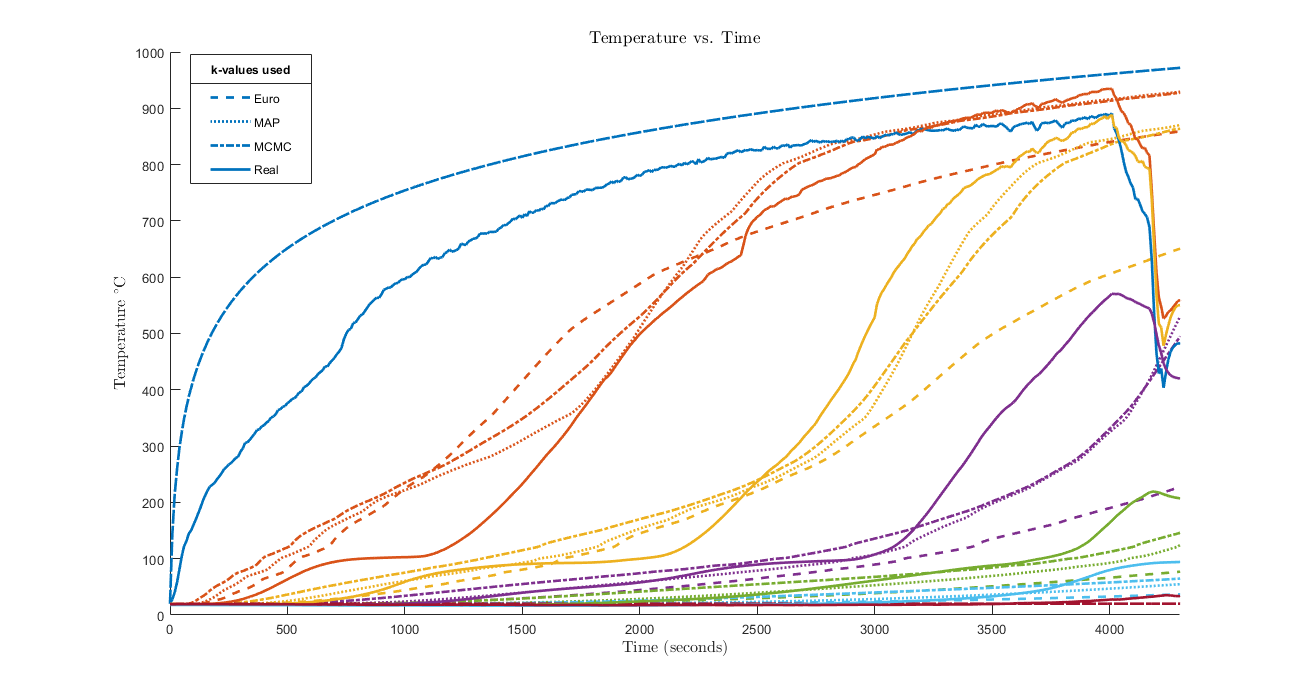
\includegraphics[width=\linewidth,]{figures/final_graph.png}
	\caption{Graph of measured data compared to model output}
	\label{final_graph}
\end{sidewaysfigure}





